\chapter{Ergebnisse}
\label{sec:ergebnisse}

Im folgenden Protokollabschnitt werden die Versuchsergebnisse der Versuchsdurchführung präsentiert.
\vspace*{-3.5mm}
\section{Sinnesprüfung}
Die aus Versuchsteil 1 wahrgenommenen Einstufungen der Abwasserproben 1 bis 3 sind in Tab. \ref{tab:optisch_sp} aufgeführt und im Vergleich mit Abb. \ref{fig:proben} nachzuvollziehen.
\vspace*{-2.5mm}
\renewcommand{\arraystretch}{1.2}
\begin{table}[h!]
	\centering
	\caption{Wahrgenommene Einstufungen der Färbung und Trübung der Abwasserproben 1 bis 3}
	\label{tab:optisch_sp}
	%\resizebox{10cm}{!}{
	\begin{tabulary}{\textwidth}{C|CCC}
		\hline
		\textbf{} & \textbf{Probe 1} & \textbf{Probe 2} & \textbf{Probe 3} \\ 
		\hline
		\textbf{Färbung} & stark gefärbt& stark gefärbt& schwach \\
		\textbf{Trübung} & undurchsichtig & undurchsichtig& klar \\
		\hline
	\end{tabulary}
	%}
\end{table}
\FloatBarrier
\vspace*{-2.5mm}

%Tabelle Ende

Für die Abwasser Proben 1 bis 3 sind die wahrgenommenen Einschätzungen zu den Gerüchen in Tab. \ref{tab:olfaktorisch_sp} aufgeführt.

\vspace*{-2.5mm}
\renewcommand{\arraystretch}{1.2}
\begin{table}[h!]
	\centering
	\caption{Wahrgenommene Einstufungen des Geruchs der Abwasserproben 1 bis 3}
	\label{tab:olfaktorisch_sp}
	%\resizebox{10cm}{!}{
	\begin{tabulary}{\textwidth}{C|CCC}
		\hline
		\textbf{} & \textbf{Probe 1} &  \textbf{Probe 2}&  \textbf{Probe 3}\\
		\hline
		\textbf{Intensität}	& schwach	&stark &ohne\\
		\textbf{Art}		& erdig, muffig	& modrig	&-\\
		\textbf{charak.-chemisch  }	& - & - & -\\
		\hline
	\end{tabulary}
	%}
\end{table}
\FloatBarrier
\vspace*{-2.5mm}

%Tabelle Ende
\vspace*{-4.5mm}
\section{Elektrochemische Ergebnisse zur Abwasserbeschaffenheit}
Die elektrochemischen Messwerte für die Abwasserproben 1 bis 3 sind in Tab. \ref{tab:elektrochemisch} eingetragen.
Zu beachten ist dabei, dass die Messwerte für den pH-Wert nur eine grobe Einschätzung liefern, da laut Messgerät die pH-Wert-Elektrode hätte gewechselt werden müssen. \\
Weitere Diskussionen zur Fehlerbetrachtung sind unter Abschnitt \ref{sec:fehler} zu finden.

\vspace*{-3.5mm}
\renewcommand{\arraystretch}{1.2}
\begin{table}[h!]
	\centering
	\caption{Elektrochemische Messwerte der Abwasserproben 1 bis 3}
	\label{tab:elektrochemisch}
	\resizebox{13cm}{!}{
	\begin{tabulary}{\textwidth}{L|C|C|C}
		\hline
		\textbf{} 						& \textbf{pH-Wert\protect\footnotemark[1] $\boldsymbol{\left[-\right]}$} & \textbf{Leitfähigkeit $\boldsymbol{\left[\si{\milli \siemens \per \centi \meter}\right]}$}& \textbf{Temperatur} $\boldsymbol{\left[\si{\celsius}\right]}$\\
		\hline
		\textbf{Probe 1}				& 1,70	& 10,59	& 17,5	\\
		\textbf{Probe 1 (filtr.)}		& 1,68  & 10,32	& 17,6	\\
		\hline
		\textbf{Probe 2}				& 7,38 	& 2,67	& 17,4	\\
		\textbf{Probe 2 (filtr.)}		& 7,58	& 2,55	& 17,8	\\
		\hline
		\textbf{Probe 3}				& 7,44	& 2,43	& 17,4	\\
		\textbf{Probe 3 (filtr.)}		& 7,54	& 2,27	& 17,9	\\
		\hline
	\end{tabulary}
	}
\end{table}
\FloatBarrier
\vspace*{-2.5mm}

%Tabelle Ende


\footnotetext[1]{pH-Wert-Elektrode auf \SI{25}{\celsius} kalibriert}


\newpage 

\section{Foto- bzw. kolorimetrische Messungen zur Abwasserbeschaffenheit}
Die für die fotometrischen bzw. kolorimetrischen Messungen erhobenen Daten lassen sich für die Abwasserproben 1 bis 3 in Tab. \ref{tab:fotometrisch} wiederfinden. In dieser Tabelle sind sowohl die Schnelltestergebnisse (ST) als auch die Reflektometerergebnisse (RM) aufgeführt. \\
Ebenfalls aufgeführt ist die Berechnung der Konzentration an Nitrat \ce{NO3-} mittels Schnelltest für Probe 1, da der Messbereich von maximalen \SI{500}{\milli \gram \per \liter} nicht ausreicht. Die dafür nötige Berechnung der Verdünnung der Probe 1 ist ab Gleichung \ref{gl1} gezeigt.

\vspace*{-3.5mm}
\renewcommand{\arraystretch}{1.2}
\begin{table}[h!]
	\centering
	\caption{Foto-/kolorimetrisch Messwerte der Abwasserproben 1 bis 3}
	\label{tab:fotometrisch}
	\resizebox{14.5cm}{!}{
	\begin{tabulary}{1.2\textwidth}{L|C|C|C}
		\hline
		\textbf{} 						& \textbf{Probe 1} $\boldsymbol{\left[\si{\milli \gram \per \liter}\right]}$& \textbf{Probe 2}$\boldsymbol{\left[\si{\milli \gram \per \liter}\right]}$&\textbf{Probe 3}$\boldsymbol{\left[\si{\milli \gram \per \liter}\right]}$\\
		\hline
		\textbf{Nitrit \ce{NO2-} (Schnelltest)}	& 2	& 0&2\\
		\textbf{Nitrit \ce{NO2-} (Reflektometer)} & <0,3  & <0,3	&<0,3\\
		\hline
		\textbf{Nitrat \ce{NO3-} (ST)}			& >500 	& 0	&0\\
		\textbf{Nitrat \ce{NO3-} (RM)}	{\footnotesize (verdünnt/unverdünnt)}		& 48/480	& <3	&7,4\\
		\hline
		\textbf{Phosphat \ce{PO4^3-} (ST)}		& {\footnotesize kein Messwert}\protect\footnotemark[2]	& 0	&25\\
		\textbf{Phosphat \ce{PO4^3-} (RM)}		& {\footnotesize kein Messwert}\protect\footnotemark[2]	& 12	&27\\
		\hline
		\textbf{Ammonium \ce{NH4+} (RM)}		& {\footnotesize kein Messwert}\protect\footnotemark[2]		&	1,3	&0,6\\
		\hline
	\end{tabulary}
	}
\end{table}
\FloatBarrier
\vspace*{-3.5mm}

%Tabelle Ende

\footnotetext[2]{keine Messung möglich, da laut Packungsbeilage  der pH-Wert zu niedrig für ein verwertbares Ergebnis ist}

\subsubsection{\underline{Verdünnung für Nitrat-Gehaltbestimmung der Probe 1}}
\textbf{Es wird von $\boldsymbol{V_{\text{Probe 1}} = \SI{100}{\milli \liter}}$ ausgegangen:}
\begin{flalign}
\label{gl1}
	\frac{\SI{500}{\milli \gram \per \liter}}{\SI{50}{\milli \gram \per \liter}} &= \frac{\SI{100}{\milli \liter}}{V_{\text{zu verdünnen}}}\\[2mm]
	V_{\text{zu verdünnen}}	&= \SI{100}{\milli \liter}*\frac{\SI{50}{\milli \gram\per \liter}}{\SI{500}{\milli \gram\per \liter}}\\[-2mm]
			&=\underline{ \SI{10}{\milli \liter}} \\[3mm]
			V_{\ce{H2O}}	&= \SI{100}{\milli \liter}-V_{\text{zu verdünnen}}\\
					&=\SI{100}{\milli \liter}-\SI{10}{\milli \liter}\\
					&= \underline{\SI{90}{\milli \liter}}\\[3mm]
	\frac{\SI{10}{\milli \liter}}{\SI{100}{\milli \liter}}	&=\frac{1}{10}\\
					&=\underline{\underline{1:10}} \quad \text{{\footnotesize (Verdünnung)}}
\end{flalign}

Mit \SI{50}{\milli \gram \per \liter} ist der Messbereich des Schnellteststreifens für Nitrat mit \SI{0}{}-\SI{500}{\milli \gram \per \liter} gut erfasst und das Volumen von \SI{10}{\milli \liter} ist einfach mittels Messzylinder abzumessen.\\
Daraus folgt eine Verdünnung von 1:10 mit einem Volumenteil (\SI{10}{\milli \liter}) Abwasserprobe 1 und neun Volumenteilen (\SI{90}{\milli \liter}) destilliertes Wasser.\\

\newpage

Der Messwert des Reflektometers für die verdünnte Lösung der Probe 1 ergibt für den Nitratgehalt \SI{48}{\milli \gram \per \liter} (siehe Tab. \ref{tab:elektrochemisch}). Hochgerechnet auf die unverdünnte Lösung ergibt sich:
\begin{flalign}
	\frac{c_{1,\text{verdünnt}}}{c_{1,\text{unverdünnt}}}	&= \frac{1}{10}\\
	c_{1,\text{unverdünnt}} &= 10*c_{1,\text{verdünnt}}\\
						&= 10*\SI{48}{\milli \gram \per \liter}\\
						&=\underline{\underline{ \SI{480}{\milli \gram \per \liter}}}
\end{flalign} 

\subsubsection{\underline{Bestimmung des anorganisch gebundenen Gesamtstickstoffs}}
Der gesamte anorganisch gebundene Stickstoff kann über den Masseanteil des Elementaren Stickstoffs an den einfachen anorganischen Verbindungen Nitrat-, Nitrit- und Ammoniumionen berechnet werden.\\
Dabei kann aus dem Massenanteil des Stickstoffs am Molekül abgeleitet werden, dass $\SI{1}{\milli\gram\per\liter}$Ammoniumionen $\frac{7}{9}\si{\milli\gram\per\liter}$ anorganisch gebundenem Stickstoff entsprechen.(vgl. Gleichung 5.1)
\begin{flalign}
\frac{M(N)}{M(\ce{NO_3^-})} &= \frac{\SI{14}{\gram\per\mole}}{\SI{14}{\gram\per\mole}+3*\SI{16}{\gram\per\mole}} =\frac{7}{31} \approx 22,6\% \\
\frac{M(N)}{M(\ce{NO_2^-})} &= \frac{\SI{14}{\gram\per\mole}}{\SI{14}{\gram\per\mole}+2*\SI{16}{\gram\per\mole}} =\frac{7}{23}\approx 30,4\%\\
\frac{M(N)}{M(\ce{NH_4^+})} &= \frac{\SI{14}{\gram\per\mole}}{\SI{14}{\gram\per\mole}+4*\SI{1}{\gram\per\mole}} =\frac{7}{9} \approx 70,0\% 
\end{flalign}

Zur Berechnung des anorganisch gebundenen Gesamtstickstoffs können die Ionenkonzentrationen mit den entsprechenden Umrechnungsfaktoren aufsummiert werden. Beispielhaft wird $N_{ges}$ für Probe 2 mit den Reflektometerergebnissen vorgerechnet, zu sehen in den Gleichungen \ref{gl:tin1} bis \ref{gl:tin2}. Die restlichen Werte des $N_{ges}$ sind in Tab. \ref{tab:tin} dargestellt.
\begin{flalign}
\label{gl:tin1}
	N_{ges,i} 	&= c_{(i,\ce{NO3^-})}*22,6\%+c_{(i,\ce{NO2^-})}*30,4\%+c_{(i,\ce{NH4^+})}*70,0\%\\[2mm]
			&= \SI{7,4}{\milli\gram\per\liter}*22,6\%+\SI{0,3}{\milli\gram\per\liter}*30,4\%+\SI{0,6}{\milli\gram\per\liter}*70,0\%\\
			&= \SI{1,67}{\milli\gram\per\liter}+\SI{0,09}{\milli\gram\per\liter}+\SI{0,42}{\milli\gram\per\liter}\\
\label{gl:tin2}
	N_{ges,3}	&=\underline{\underline{\SI{2,18}{\milli\gram\per\liter}}}
\end{flalign}

\vspace*{-8.5mm}
\renewcommand{\arraystretch}{1.2}
\begin{table}[h!]
	\centering
	\caption{$N_{ges}$ der Abwasserproben 1 bis 3}
	\label{tab:tin}
	%\resizebox{10cm}{!}{
	\begin{tabulary}{1.2\textwidth}{C|C|C|C}
		\hline
		\textbf{} 						& \textbf{Probe 1} & \textbf{Probe 2}&\textbf{Probe 3}\\
		\hline
		\textbf{$N_{ges}$ $\boldsymbol{\left[\si{\milli \gram \per \liter}\right]}$}	& 108,67\protect\footnotemark[3] & 0,77 & 2,18\\
		\hline
	\end{tabulary}
	%}
\end{table}
\FloatBarrier
\vspace*{-2.5mm}

%Tabelle Ende
\footnotetext[3]{zweifelhaftes Ergebnis, da kein Messwert für den Ammoniumgehalt vorhanden ist}

\newpage

\subsection*{\underline{Bestimmung des gebundenen Gesamtphosphors}}
Die Bestimmung des gebundenen Gesamtphosphors folgt analog der Bestimmung des Gesamtstickstoffs:
\begin{flalign}
\frac{M(P)}{M(\ce{PO_4^3-})} &= \frac{\SI{31}{\gram\per\mole}}{\SI{31}{\gram\per\mole}+4*\SI{16}{\gram\per\mole}} =\frac{31}{95} \approx 32,6\% 
\end{flalign}

Beispielhaft für Reflektometerergebnisse der Probe 3 vorgerechnet:
\begin{flalign}
P_{ges,i}	&= c_{(i,\ce{PO4^3-})}*32,6\% \\[2mm]
P_{ges,3}	&= \SI{27}{\milli \gram \per \liter}*32,6\%\\[2mm]
		&= \underline{\underline{\SI{8,8}{\milli \gram \per \liter}}}
\end{flalign}

\vspace*{-8.mm}
\renewcommand{\arraystretch}{1.2}
\begin{table}[h!]
	\centering
	\caption{$P_{ges}$ der Abwasserproben 1 bis 3}
	\label{tab:tp}
	%\resizebox{10cm}{!}{
	\begin{tabulary}{1.2\textwidth}{C|C|C|C}
		\hline
		\textbf{} 						& \textbf{Probe 1} & \textbf{Probe 2}&\textbf{Probe 3}\\
		\hline
		\textbf{$P_{ges}$ $\boldsymbol{\left[\si{\milli \gram \per \liter}\right]}$}	& {\footnotesize kein Ergebnis\protect\footnotemark[4]} & 3,9 & 8,8\\
		\hline
	\end{tabulary}
	%}
\end{table}
\FloatBarrier
\vspace*{-5.5mm}
%Tabelle Ende
\footnotetext[4]{kein Ergebnis, da kein Messwert für den Phosphatgehalt vorhanden ist}

%\newpage

\section{Gegenüberstellung der Mindestanforderungen für das Einleiten kommunaler Abwässer in einen Vorfluter der GK 5 mit den Abwasserproben}
Die Referenzwerte der Mindestanforderungen für das Einleiten kommunaler Abwässer in den Vorfluter der Größenklasse 5 sind im Anhang von \cite[S. 29]{Skript} zu finden.
\begin{figure}[h!]
	\begin{tikzpicture}
	\selectcolormodel{gray}
	\begin{axis}[
	xbar=1pt,% space of 0pt between adjacent bars
	bar width=7,
	width=15cm,
	height=7cm,
	%minor y tick num=4,
	xmax=110,xmin=0,
	x tick label style={/pgf/number format/.cd,%
		scaled x ticks = false,
		set decimal separator={,},
		fixed},
	symbolic y coords={Probe 3,Probe 2,Probe 1\protect\footnotemark[5],max. für GK 5},
	ytick=data,
	%legend style={at={(0.5,-0.15)},
	%	anchor=north,legend columns=-1},
	xtick={0,10,...,110},
	grid=major,
	xlabel=Gehalt in  \si{\milli\gram\per\liter},
	%enlargelimits=0.15,
	%postaction={pattern=north east lines}
	]
	%NH4-N
	\addplot[pattern=north east lines] coordinates {
		(0,Probe 1\protect\footnotemark[5]) (1.3,Probe 2) (0.6,Probe 3) (10,max. für GK 5)
	};
	%N gesamt
	\addplot coordinates {
		(108,Probe 1\protect\footnotemark[5]) (0.77,Probe 2) (2.18,Probe 3) (13,max. für GK 5)
	};
	%P gesamt
	\addplot[fill=black] coordinates {
		(0,Probe 1\protect\footnotemark[5]) (3.9,Probe 2) (8.8,Probe 3) (1,max. für GK 5) 
	};
	\legend{$NH_4-N$,$N_{ges}$,$P_{ges}$}
	\end{axis}
	\end{tikzpicture}
	\caption{Vergleich mit Mindestanforderungen für das Einleiten kommunaler Abwässer in den Vorfluter der GK 5 für die Abwasserproben 1 bis 3}
	\label{Balkendiagramm}
\end{figure}
\FloatBarrier
\footnotetext[5]{kein Messwert für Phosphat- bzw. Ammoniumgehalt vorhanden}

%\vspace*{-2.5mm}
\renewcommand{\arraystretch}{1.2}
\begin{table}[h!]
	\centering
	\caption[Tabellarischer Vergleich der Messwerte mit den Mindestanforderungen für das Einleiten kommunaler Abwässer in den Vorfluter der GK 5]{Tabellarischer Vergleich der Messwerte mit den Mindestanforderungen für das Einleiten kommunaler Abwässer in den Vorfluter der GK 5 \cite[S. 29]{Skript}}
	\label{tab_vgl}
	%\resizebox{10cm}{!}{
	\begin{tabulary}{1.2\textwidth}{l|C|C|C}
		\hline
		 & \textbf{$NH_4^+-N$} $\boldsymbol{\left[\si{\milli\gram\per\liter}\right]}$& \textbf{$N_{ges}$}$\boldsymbol{\left[\si{\milli\gram\per\liter}\right]}$&\textbf{$P_{ges}$}$\boldsymbol{\left[\si{\milli\gram\per\liter}\right]}$\\
		\hline
		\textbf{Grenzwert} & \textbf{10} & \textbf{13} & \textbf{1} \\
		\hline
		Probe 1 & {\footnotesize kein Messwert\protect\footnotemark[5]} & 108,67 & {\footnotesize kein Messwert\protect\footnotemark[5]} \\
		Probe 2 & 1,3 & 0,77 & 3,9 \\
		Probe 3 & 0,6 & 2,18 & 8,8 \\
		\hline
	\end{tabulary}
	%}
\end{table}
\FloatBarrier

\footnotetext[5]{kein Messwert für Phosphat- bzw. Ammoniumgehalt vorhanden}

\section{Gegenüberstellung der durchschnittlichen Beschaffenheit von häuslichem Abwasser mit den Abwasserproben}

Um die Messwerte des Versuches mit häuslichem Abwasser gegenüberzustellen wird die Tabelle Tab. \ref{tab:komm} (siehe \cite[S. 29]{Skript}) genutzt.

\vspace*{-2.5mm}
\renewcommand{\arraystretch}{1.2}
\begin{table}[h!]
	\centering
	\caption[Tabellenausschnitt zur durchschnittlichen Beschaffenheit von häuslichem Abwasser]{Tabellenausschnitt zur durchschnittlichen Beschaffenheit von häuslichem Abwasser \cite[S. 29]{Skript}}
	\label{tab:komm}
	%\resizebox{10cm}{!}{
	\begin{tabulary}{1.2\textwidth}{l|C|C|C|C}
	\textbf{Kriterium} & \textbf{Maßeinheit} &\multicolumn{3}{c}{\textbf{Belastungsgrad}}\\
	\hline
			&		&	gering&mittel &stark\\
	\hline
	pH-Wert	& - & 6,6&7,6&8,6\\
	$N_{ges}$&	\si{\milli \gram \per \liter} & 20&50&85\\
	$P_{ges}$&	\si{\milli \gram \per \liter} & 7&20&30\\
	\end{tabulary}
	%}
\end{table}
\FloatBarrier
\vspace*{-8mm}

\begin{figure}[h!]
	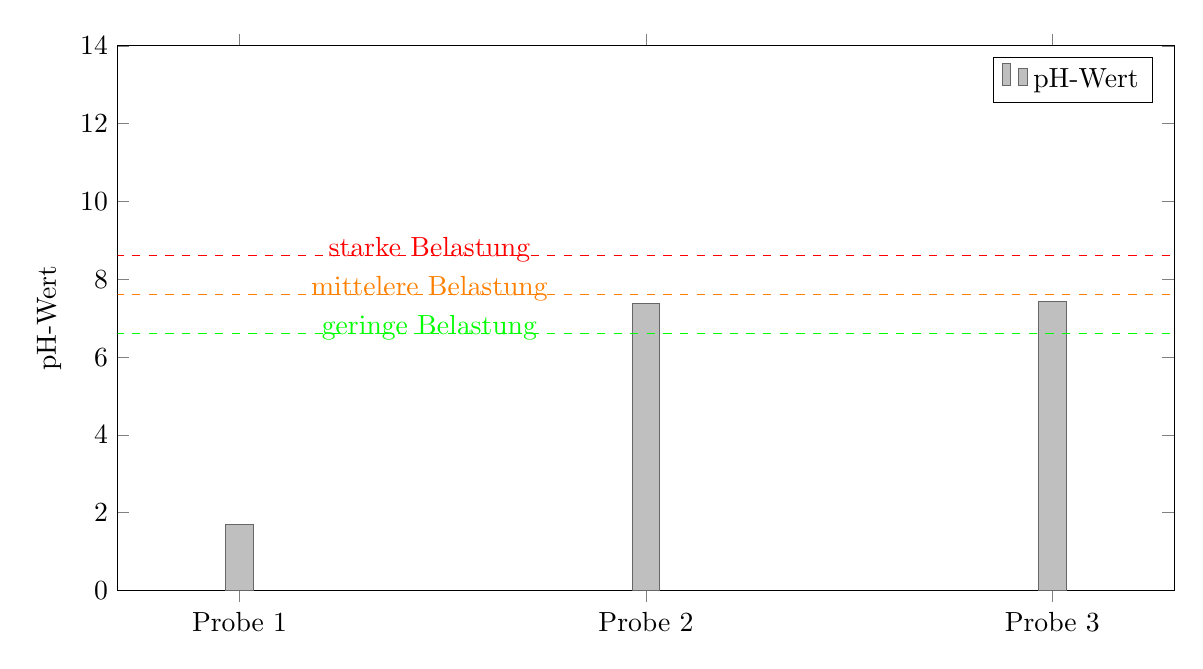
\begin{tikzpicture}
	\begin{axis}[
	%x tick label style={
	%	/pgf/number format/1000 sep=},
	xtick = data,
	ylabel=pH-Wert,
   	enlarge x limits=0.15,
	ybar,
	ymin = 0,
	ymax = 14,
	bar width=10pt,
	width=15cm,
	height=8.5cm,
	symbolic x coords={0,Probe 1, Probe 2,Probe 3,2,1},
	]
	\addplot[fill=gray!50,draw=black!60] coordinates {(Probe 1,1.7) (Probe 2,7.38) (Probe 3,7.44)};
	\addplot[green,sharp plot,update limits=false, dashed] 
	coordinates {(0,6.6) (1,6.6)} 
	node[above] at (axis cs:Probe 2,6.2) {\hspace*{-5.5cm}geringe Belastung};
	\addplot[orange,sharp plot,update limits=false, dashed] 
	coordinates {(0,7.6) (1,7.6)} 
	node[above] at (axis cs:Probe 2,7.2) {\hspace*{-5.5cm}mittelere Belastung};
	\addplot[red,sharp plot,update limits=false, dashed] 
	coordinates {(0,8.6) (1,8.6)} 
	node[above] at (axis cs:Probe 2,8.2) {\hspace*{-5.5cm}starke Belastung};
	\legend{pH-Wert}
	\end{axis}
	\end{tikzpicture}
	\caption{pH-Wert-Beschaffenheit der Abwasserproben 1 bis 3}
	\label{ph}
\end{figure}
\FloatBarrier

\pagebreak

\begin{figure}[h!]
	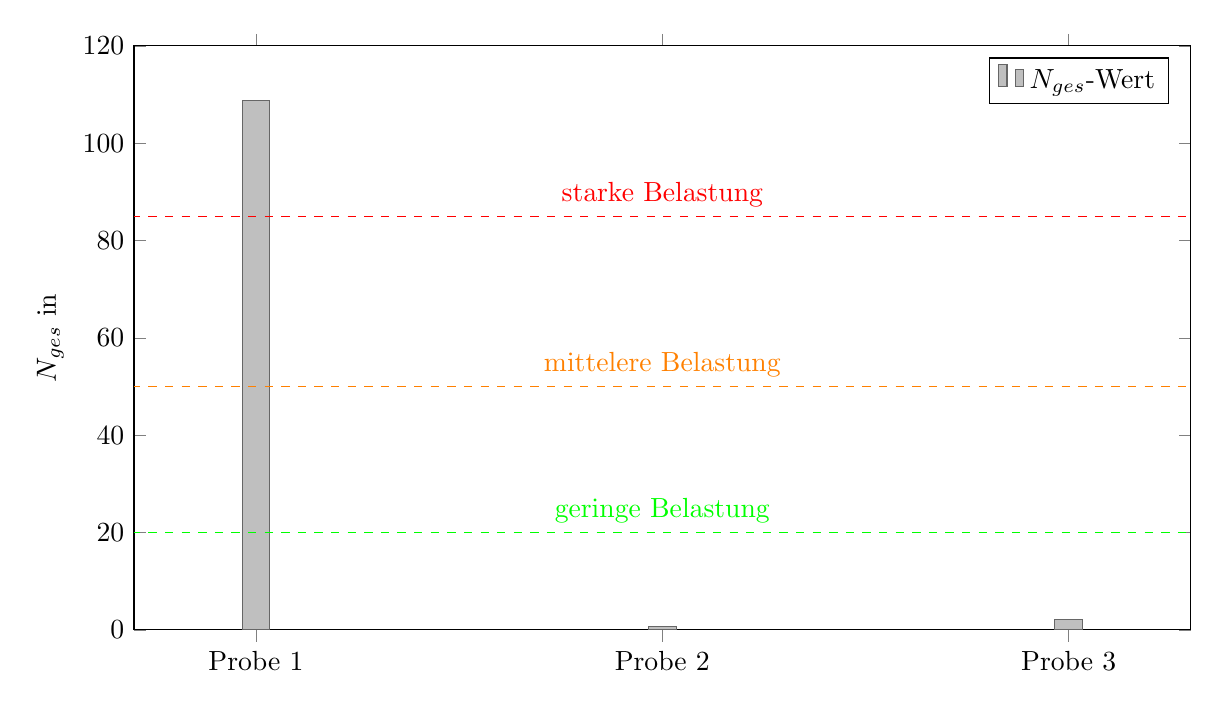
\begin{tikzpicture}
	\begin{axis}[
	%x tick label style={
	%	/pgf/number format/1000 sep=},
	xtick = data,
	ylabel=$N_{ges}$ in \si{\milli \gram \per \liter},
	enlarge x limits=0.15,
	ybar,
	ymin = 0,
	ymax = 120,
	bar width=10pt,
	width=15cm,
	height=9cm,
	symbolic x coords={0,Probe 1, Probe 2,Probe 3,2,1},
	]
	\addplot[fill=gray!50,draw=black!60] coordinates {(Probe 1,108.7) (Probe 2,0.77) (Probe 3,2.18)};
	\addplot[green,sharp plot,update limits=false, dashed] 
	coordinates {(0,20) (1,20)} 
	node[above] at (axis cs:Probe 2,20) {geringe Belastung};
	\addplot[orange,sharp plot,update limits=false, dashed] 
	coordinates {(0,50) (1,50)} 
	node[above] at (axis cs:Probe 2,50) {mittelere Belastung};
	\addplot[red,sharp plot,update limits=false, dashed] 
	coordinates {(0,85) (1,85)} 
	node[above] at (axis cs:Probe 2,85) {starke Belastung};
	\legend{$N_{ges}$-Wert}
	\end{axis}
	\end{tikzpicture}
	\caption{$N_{ges}$-Beschaffenheit der Abwasserproben 1 bis 3}
	\label{nges}
\end{figure}
\FloatBarrier

\vspace*{3cm}

\begin{figure}[h!]
	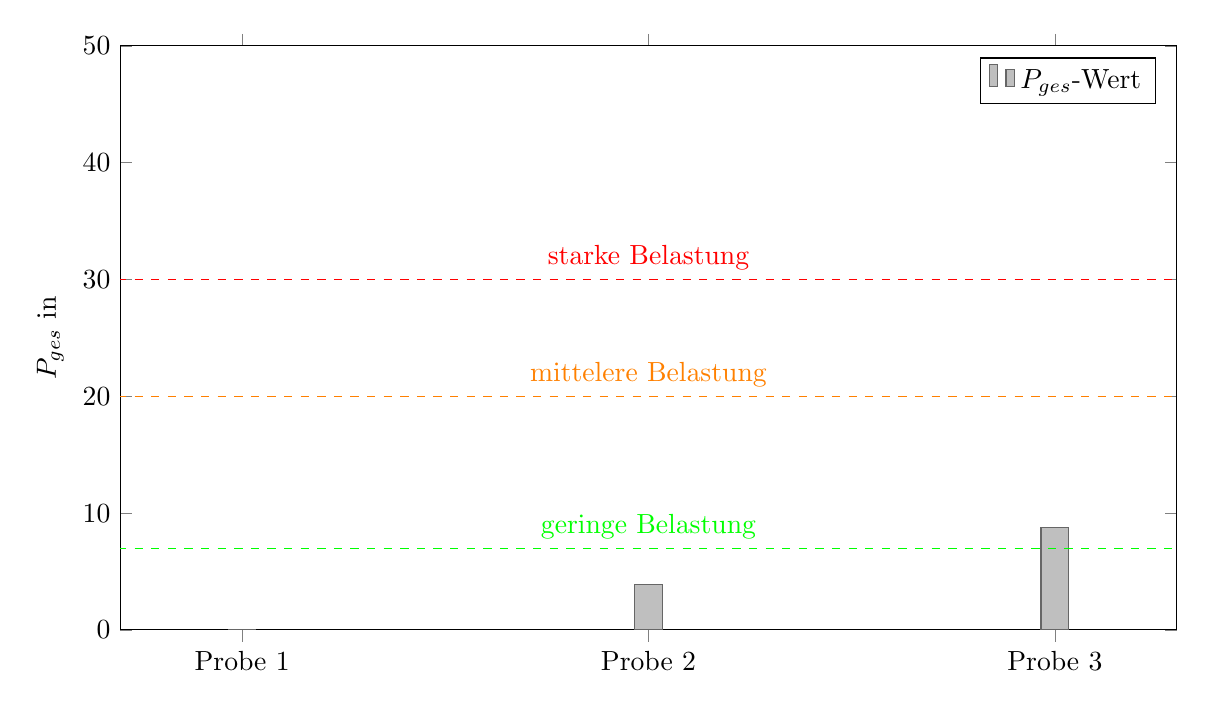
\begin{tikzpicture}
	\begin{axis}[
	%x tick label style={
	%	/pgf/number format/1000 sep=},
	xtick = data,
	ylabel=$P_{ges}$ in \si{\milli \gram \per \liter},
	enlarge x limits=0.15,
	ybar,
	ymin = 0,
	ymax = 50,
	bar width=10pt,
	width=15cm,
	height=9cm,
	symbolic x coords={0,Probe 1, Probe 2,Probe 3,2,1},
	]
	\addplot[fill=gray!50,draw=black!60] coordinates {(Probe 1,0) (Probe 2,3.9) (Probe 3,8.8)};
	\addplot[green,sharp plot,update limits=false, dashed] 
	coordinates {(0,7) (1,7)} 
	node[above] at (axis cs:Probe 2,7) {geringe Belastung};
	\addplot[orange,sharp plot,update limits=false, dashed] 
	coordinates {(0,20) (1,20)} 
	node[above] at (axis cs:Probe 2,20) {mittelere Belastung};
	\addplot[red,sharp plot,update limits=false, dashed] 
	coordinates {(0,30) (1,30)} 
	node[above] at (axis cs:Probe 2,30) {starke Belastung};
	\legend{$P_{ges}$-Wert}
	\end{axis}
	\end{tikzpicture}
	\caption{$P_{ges}$-Beschaffenheit der Abwasserproben 1 bis 3}
	\label{pges}
\end{figure}
\FloatBarrier

